\documentclass[12pt, a4paper, french, BCOR = 0pt, DIV = 10]{scrartcl}
\usepackage{graphicx} % Required for inserting images
\usepackage{babel}
\usepackage{amsmath}
\usepackage[utf8]{inputenc}
\usepackage[T1]{fontenc}
\usepackage{graphicx}
\graphicspath{ {./images/} }

\usepackage{bigints}

\usepackage{pxfonts}

\title{MIG Verre - Modélisation des fours}
\author{\small{Simon Lamaze - Corto Beck - Girardet Grégoire -Fraenkel Paul}}

\begin{document}
	
	\maketitle
	
	\section{Introduction}
	\raggedright
	Ce mini-projet traite de la modélisation et de l'optimisation énergétique des fours à verre.  La compréhension des phénomènes physiques qui prennet place dans un four est essentielle à l'optimisation des procédés de fusion, et à la mise en place d'une simulation numérique. \\ [0.5 cm]
	Voici un four à fusion:
	

	
	
	
	
	\section{ Déroulement de la simulation}
	\raggedright
	Tâche 1 : positionnement du problème : \\
	Il nous faut tout d'abord définir l'environnement du problème physique, à savoir, les équations régissant domaine liquide, les conditions limites de ce domaine pour modéliser l'interaction avec l'extérieur, et les conditions initiales. \\[0.3 cm]
	
    Tâche 2: prise en main des outils de calcul\\
	Les calculs de la modélisation ont été réalisés sur cluster de calcul Laffite du CEMEF, avec le logiciel Cimlib. Cet environnement nécessite plusieurs étapes de modélisation : création de la géométrie du four, et maillage, écriture de la maquette de la simulation, envoi sur le cluster, puis post-traitement.\\ [0.3 cm]
	
	Tâche 3 : Calcul sur un cas à voûte chaude\\ 
	Une fois les calculs maîtrisés, nous réalisons une simulation d'un four à voûte chaude jusqu'à obtenir un cas convergé. Nous avons ensuite réalisé un bilan énergétique \\ [0.3 cm]
	
	Tâche 4 : Calcul sur un cas à voûte plus froide \\ 
    Les mêmes calculs sont réalisés pour une température de voûte plus froide, compensée par un apport énergétique des électrodes.\\ [0.3 cm]
	
	Tâche 5: Bilan du gain énergétique et des émissions carbone\\
    Les résultats des simulations précédentes permettent de réaliser le bilan énergétique et de quantifier les émissions de carbone\\ [0.5cm]
	
	
	On  utilise le logiciel Paraview pour visualiser les résultats.
	Visualiser la propagation d'un champ pour définir le temps de résidence.
	Faire plusieurs calculs avec des tailles différentes.
	
	\section{Positionnement du problème}
	Les équations et approximations que nous avons choisies qui régissent le système sont les suivantes : \\
	\subsection{ Equations de Navier-Stokes et thermique }
    - Conservation de la masse :
    $$\vec{\nabla}\cdot \vec(u)=0$$

    - Conservation du moment :
    $$\rho_{0} \frac{D\vec{V}}{Dt} = -\rho_{0} \beta (T-T_{0}) \vec{g} + \vec {\nabla} . [ 2 \eta (T) \vec{E}] - \vec {\nabla} P$$

    - Equation de la chaleur :
    $$\rho C_{p} \frac{DT}{Dt} = \vec {\nabla} .  (\lambda_{eq}(T) \vec{\nabla} T ) + \sigma_{e}(T) (\vec \nabla\phi)^2 - \rho\Delta H_{r} \frac{d\alpha}{dT}$$
    
	Comme les transferts de chaleur sous formes radiatives sont très importants, on ne peut pas les négliger dans l'équation habituelle de diffusion de la chaleur: $ \rho C_{p} \frac{\partial T}{\partial t} = - \vec{\nabla} . (\lambda\vec{\nabla}T) $. Cependant, comme le milieu est semi-transparent, on peut utiliser l'approximation de Rosseland qui consiste à approximer le terme de flux radiatif $\vec{q_r}$ par un transfert thermique de fourier de conductivité thermique $\lambda_{r} = \frac{16n² \sigma T^{3}}{3\beta_{R}} $. On définit alors $\lambda_{eq} = \lambda + \lambda_r$
	\\ [0.5 cm]
	
	\subsection{Puissance électrique}
	\raggedright
    L'apport de puissance électrique par les électrodes peut être réalisé sous deux fonctionnements : uniphasé ou triphasé.
	On se place dans un premier temps dans le cas uniphasé :\\ [0.2 cm ]
    L'effet joule volumique est donnée par l'équation suivante :
    $$ d^3P_{eq} = \sigma_{e}(T)(\vec \nabla\phi \cdot \vec \nabla\phi) = \sigma_{e}(T)(\vec \nabla\phi)^2$$
    Sur l'ensemble du volume du système, on obtient alors la puissance électrique totale : 
	$$P_{eq}=\int_\Omega \sigma_{e}(T)(\vec \nabla\phi)^2~dV  = \int_\Omega \vec \nabla[\sigma_{e}(T)\vec \nabla\phi]~dV $$\\
	\raggedright
	Par intégration par partie et loi de conservation du potentiel ($ \vec{\nabla}^2 \phi = 0 $). Le théorème de Green-Ostrogradski donne: 
	
	$$ P_{eq}=\phi_{elec} \int_{\partial electrode} \sigma_{e}(T)\vec \nabla\phi \cdot \vec{n}~dS\ $$
    
	Car le potentiel $\phi$ est constant $\phi=\phi_{elec} $ à la frontière des électrodes. \\

    Dans le cas de l'industrie, on utilise plus souvent un courant triphasé dans un triplet d'électrodes. Pour prendre en compte ce déphasage, on utilise des potentiels complexes, pour lesquels on résoud les équations précedentes sur le champe réel et le champ complexe.

    
	\subsection{ Expressions des différentes grandeurs et constantes}
    Plusieurs paramètres du verres varient avec la température, et il convient de modéliser ces variations.\\ [0,5 cm]
	
	- On modélise la dépendance de la viscosité à la température par une loi de type VFT ( Vogel-Fulcher-Tamman) \\
	$$
	\eta (T)  = 10^{A_{\eta}} e^{\frac{ln(10) B}{T-T_{\eta}}} ~~~~~~~~~ log(\eta) = A_{\eta} + \frac{B}{T-T_{\eta}}
	$$\\ [0,5 cm]

    
	Le taux de conversion $\alpha$ est une sigmoïde : fonction d'erreur de Gauss\\ [0.3cm]
	
	
	\raggedright
	- La dépendance de la masse volumique est :
	$$ \rho(T) = \rho_{0}  (1 - \beta \Delta T) $$
    \setlength{\parindent}{20pt}
    Avec : \\
    $\beta = -\frac{1}{\rho_{0}} \frac{d\rho}{dt}$\\
    $\Delta T = T-T_0$\\
    $T_0, \rho_0$ : (resp.) température et masse volumique de références\\[0.5 cm]
	\setlength{\parindent}{0pt}
	
	
	- La dépendance de la conductivité électrique est :
    $$ \sigma_{e} (T) =  A_{e} e^{\frac{-B_{e}}{T}}	$$
    \setlength{\parindent}{20pt}
    Avec :\\
    $A_e,B_e$ : Coefficients de la loi d'Arrhénius\break\\[0.5 cm]
    \setlength{\parindent}{0pt}
    
	- Dérivée particulaire : \\
	$$ \frac{DG}{Dt}=\frac{\partial G}{\partial t} + (\vec {v} \cdot \vec {\nabla } ) G
	$$\\[0.5cm]
	
	
	
	- Le calcul tu temps de résidence dans le four est particulièrement important car il conditionne la qualité de la fusion, en réduisant la quantité de bulles ou la présence d'infondus. Une première méthode consiste à étudier la réponse à un Dirac d'apport en matière dans le four en observant le flux de matière à la sortie au cours du temps. Le flux pondéré d'un scalaire C à travers la surface de sortie est donné par :\\[0.3 cm]
	$$
	\phi_{C} =  \iint_S C\vec{u} \cdot \vec{n}~dS  ~~~~~~~~~~ \phi = \iint_S \vec{u} \cdot \vec{n}~dS  ~~~~~~~~~~
	\langle C \rangle = \frac{\phi_{C}}{\phi}
	$$ 
	\\ [0.5 cm]
	Néanmoins, il est plus aisé de calculer la réponse à un échelon, ce qui implique que la distribution des temps de résidence, à savoir la réponse à un dirac, est alors donnée par \[E(t)=\frac{d\langle C \rangle}{dt}\]
	
	\subsection{État aux frontières}
	
	Les flux thermiques sont donnés par les lois de Newton et Stefan aux parois et surfaces libres. Le batch (matière d'entrée) est introduit à iso température. On considère les transfert thermiques de Boltzmann uniquement pour la surface libre.
	On peut calculer les flux aux frontières par la loi de Newton sur les transferts conducto-convectifs.\\ 
	\centering
	$$
	\phi_{wall} = h_{wall} (T - T_{\infty}) ~~~~~~~~	
	\phi_{haut} = h_{haut} (T - T_{haut}) + \epsilon \sigma (T^4 - T_{haut}^4)
	$$
    \raggedright
    $\epsilon : $\break
    $\sigma_{SB}$ : Constante\ de\ Stefan-Boltzman
    \\[0.5 cm]
    Il est possible de définir la température $T_{haut}$ comme une constante sur l'ensemble de la surface libre. Néanmoins, le chauffage par flamme dans un four industriel présente une hétérogénéité de cet apport calorifique, avec généralement une température plus important au centre. Bien qu'il serait théoriquement possible de réaliser une simulation CFD de la dynamique du gaz lors de sa combustion, ceci est inenvisageable à cause du temps de calcul nécessaire. Il convient donc d'approximer cette répartition de température par une fonction constante du temps.
    $$
        T_{haut}(\vec{r}) = T_{haut, min} + \Delta T_{haut} \space e^{-||\vec{r^{\prime}}||}
    $$
    $T_{haut, min}$ : Température minimale de voûte
    \break
    $\Delta T_{haut}$ : Différence de température maximale
	
	\section{Prise en main du langage et des logiciels de visualisation}
 	\raggedright
	Apprentissage du logiciel gmsh pour définir la géométrie d'un four et calculer la maillage qui servira à appliquer la méthode aux éléments finis . Ensuite traduction en format .t , convenant au langage mtc , des fichier gmsh . 
	Connexion au cluster de calcul, prise en main du logiciel Paraview pour visualiser les résultats .
	
	Pour le script, nous avons utilisé un squelette de code fourni par F.Pigeonneau .
	
	\section{Simulations réalisées}
	
	\subsection{Première série de calculs}
	\paragraph{}
	 Disposant de 4 postes de calculs , nous avons commencé par chercher à simuler un four  d'une forme ressemblant à celle d'un four industriel .
	 
	 \paragraph{Liste des instructions:}
	 cd /work/MINES-PARISTECH/slamaze
	 sf
	 nano ihm.mtc => changer le temps à 0
	 cd GlassFurnace3D/
	 cimlib CFD driver glassfurnace3d.mtc
	 
	 ls Geometrie/
	 mv Geometrie/indicfrontieres.vtu /work/MINES-PARISTECH/slamaze/ => open avec PARAVIEW, vérifier les frontières
	 nano ihm.mtc , modifier le temps
	 sbatch job.sh// [1 cm]
	 
	 Voici la géométrie choisie du four :
	 
	 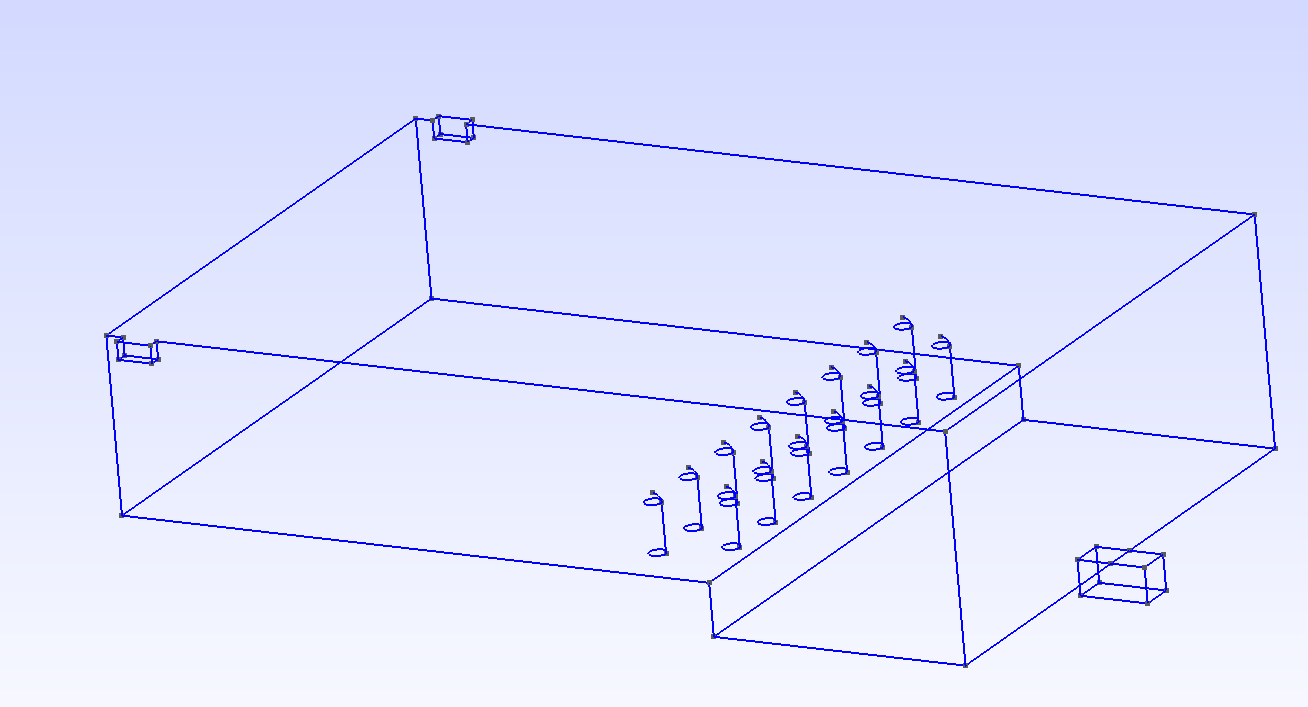
\includegraphics[scale=0.5]{Géométrie fours}
	 
	 Nous avons choisi dans un premier temps d'ajouter un mur à ce modèle, et nous avons modélisé ce four avec différents nombres d'électrodes : 15 sans mur, 3 avec mur . Les simulations se sont déroulées sur les périodes de temps que nous permettaient la puissance du cluster de calcul utilisé . \\
	 
	 Nous obtînmes alors l'évolution de différentes grandeurs , comme la puissance échangée sur la surface libre ou encore le flux pondéré de température en sortie  . \\
	 
	 \begin{align}
	 	$$P_{SurfL}= \iint_ h_{SurfL} (T_{flamme}-T)~dS ~~~~~~~~~~
	 	\langle T \rangle~~a~~\acute{e}t\acute{e}~~d\acute{e}fini~~dans~~un~~paragraphe~~pr\acute{e}c\acute{e}dent
	 	$$
	 \end{align}
	 
 
	
	
\end{document}
